\section{Toy Experiment Visualizations}
\label{app:toy_experiment}
In this section, we present visualizations of the toy experiment under each scenario. As shown in \autoref{fig:toy_vis}, when the teacher distribution exhibits low entropy, the student model converges closely to the teacher distribution. However, when the teacher distribution has high entropy, optimization using a reverse-KL-based reward causes the student to concentrate on a small number of dominant indices. As a result, the global structure of the teacher distribution is not fully captured.
\begin{figure}[H]
  \centering

  \begin{subfigure}{0.48\textwidth}
    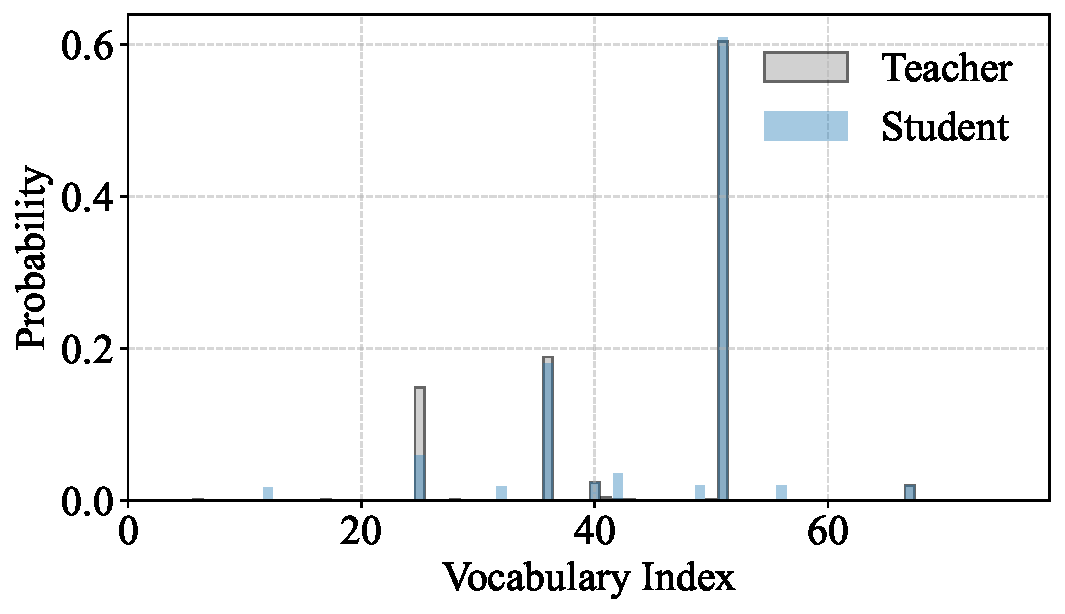
\includegraphics[width=\linewidth]{figure/toy_low.pdf}
    \caption{Low Entropy Teacher Distribution}
  \end{subfigure}
  \hfill
  \begin{subfigure}{0.47\textwidth}
    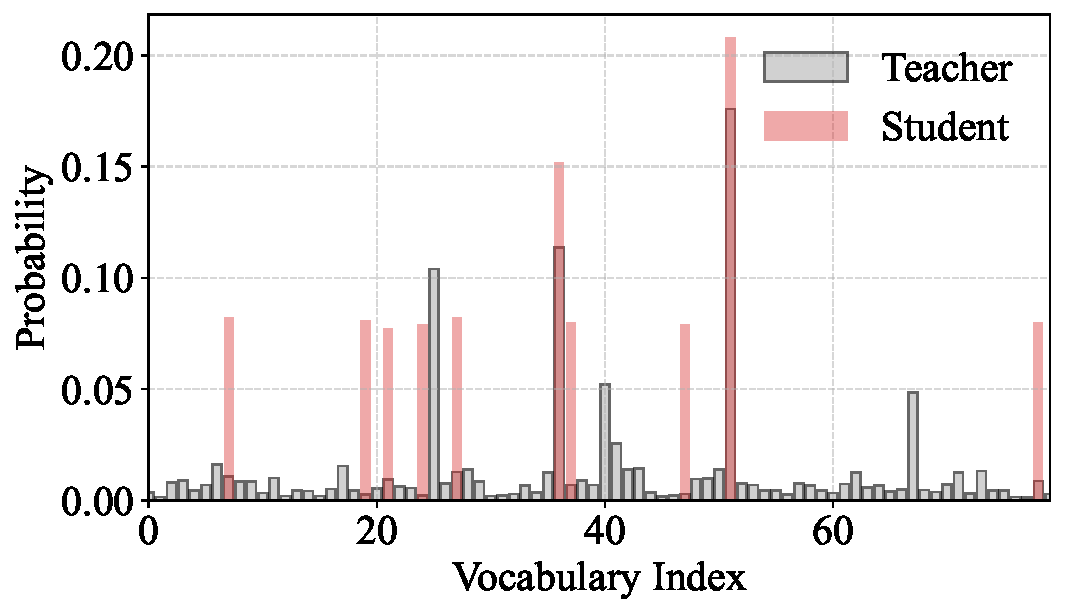
\includegraphics[width=\linewidth]{figure/toy_high.pdf}
    \caption{High Entropy Teacher Distribution}
  \end{subfigure}

  \caption{Teacher–student distributions under low and high-entropy scenarios. When the teacher distribution has low entropy, the student model accurately converges to the teacher. In contrast, when the teacher distribution has high entropy, optimization with reverse KL based reward leads the student to align with a few dominant indices of the teacher distribution, while the global structure is not fully approximated.}
  \label{fig:toy_vis}
\end{figure}